\documentclass[times,specification,annotation]{itmo-student-thesis}

%% Опции пакета:
%% - specification - если есть, генерируется задание, иначе не генерируется
%% - annotation - если есть, генерируется аннотация, иначе не генерируется
%% - times - делает все шрифтом Times New Roman, собирается с помощью xelatex
%% - languages={...} - устанавливает перечень используемых языков. По умолчанию это {english,russian}.
%%                     Последний из языков определяет текст основного документа.

%% Делает запятую в формулах более интеллектуальной, например:
%% $1,5x$ будет читаться как полтора икса, а не один запятая пять иксов.
%% Однако если написать $1, 5x$, то все будет как прежде.
\usepackage{icomma}

%% Один из пакетов, позволяющий делать таблицы на всю ширину текста.
\usepackage{tabularx}

%% Данные пакеты необязательны к использованию в бакалаврских/магистерских
%% Они нужны для иллюстративных целей
%% Начало
\usepackage{tikz}
\usetikzlibrary{arrows}
\usepackage{filecontents}
\begin{filecontents}{bachelor-thesis.bib}
@online{ graph-attention-networks,
    year        = {2018},
    title       = {Graph Attention Networks},
    author      = {\colorbox{orange}{имена не на английском}},
    url         = {https://arxiv.org/abs/1710.10903},
    year        = {2018},
    langid      = {english}
}

@online{ gated-graphs-nn,
    year        = {2018},
    title       = {Learning to Represent Programs with Graphs},
    author      = {Miltiadis Allamanis, Marc Brockschmidt, Mahmoud Khademi},
    url         = {https://arxiv.org/abs/1711.00740},
    year        = {2018},
    langid      = {english}
}

@online{ tree-gen,
    year        = {2019},
    title       = {TreeGen: A Tree-Based Transformer Architecture for Code Generation},
    author      = {Zeyu Sun, Qihao Zhu, Yingfei Xiong},
    url         = {https://arxiv.org/abs/1911.09983},
    year        = {2019},
    langid      = {english}
}

@online{ code2vec,
    year        = {2019},
    title       = {code2vec: Learning Distributed Representations of Code},
    author      = {Uri Alon, Meital Zilberstein, Omer Levy},
    url         = {https://arxiv.org/abs/1803.09473},
    year        = {2019},
    langid      = {english}
}

@online{ slm,
    year        = {2019},
    title       = {Structural Language Models of Code},
    author      = {Uri Alon, Roy Sadaka, Omer Levy},
    url         = {https://arxiv.org/abs/1910.00577},
    year        = {2020},
    langid      = {english}
}

@inproceedings{ example-english,
    year        = {2015},
    booktitle   = {Proceedings of IEEE Congress on Evolutionary Computation},
    author      = {Maxim Buzdalov and Anatoly Shalyto},
    title       = {Hard Test Generation for Augmenting Path Maximum Flow 
                   Algorithms using Genetic Algorithms: Revisited},
    pages       = {2121-2128},
    langid      = {english}
}

@article{ example-russian,
    author      = {Максим Викторович Буздалов},
    title       = {Генерация тестов для олимпиадных задач по программированию 
                   с использованием генетических алгоритмов},
    journal     = {Научно-технический вестник {СПбГУ} {ИТМО}},
    number      = {2(72)},
    year        = {2011},
    pages       = {72-77},
    langid      = {russian}
}

@article{ unrestricted-jump-evco,
    author      = {Maxim Buzdalov and Benjamin Doerr and Mikhail Kever},
    title       = {The Unrestricted Black-Box Complexity of Jump Functions},
    journal     = {Evolutionary Computation},
    year        = {2016},
    note        = {Accepted for publication},
    langid      = {english}
}

@book{ bellman,
    author      = {R. E. Bellman},
    title       = {Dynamic Programming},
    address     = {Princeton, NJ},
    publisher   = {Princeton University Press},
    numpages    = {342},
    pagetotal   = {342},
    year        = {1957},
    langid      = {english}
}
\end{filecontents}
%% Конец

%% Указываем файл с библиографией.
\addbibresource{bachelor-thesis.bib}

\begin{document}

\studygroup{M3436}
\title{Генерация Kotlin кода с помощью нейронной сети архитектуры Transformer для фаззинга компилятора}
\author{Тихонов Виталий Андреевич}{Тихонов В.А.}
\supervisor{Фильченков Андрей Александрович}{Фильченков А.А.}{канд. физ.-мат. наук}{доцент, научный сотрудник Университета ИТМО}
\publishyear{2021}
%% Дата выдачи задания. Можно не указывать, тогда надо будет заполнить от руки.
\startdate{01}{сентября}{2020}
%% Срок сдачи студентом работы. Можно не указывать, тогда надо будет заполнить от руки.
\finishdate{31}{мая}{2021}
%% Дата защиты. Можно не указывать, тогда надо будет заполнить от руки.
\defencedate{\colorbox{orange}{15}}{июня}{2021}

\addconsultant{Петухов В.А.}{без степени, без звания}

\secretary{Павлова О.Н.}

%% Задание
%%% Техническое задание и исходные данные к работе
\technicalspec{Требуется попробовать применить нейронные сети, построенные на архитектуре
Transformer для генерации кода на языке Kotlin. В архитектуру сети должна быть заложена
генерация кода не только в соответствии с грамматикой языка (правила синтаксиса), но и в
соответствие с некоторыми правилами семантики.}

%%% Содержание выпускной квалификационной работы (перечень подлежащих разработке вопросов)
\plannedcontents{\begin{enumerate}
    \item Провести обзор существующих архитектур нейронных сетей Transformer и сделать
аргументированный выбор трансформера для генерации кода.
    \item Изучить существующие способы делать code embedding и выбрать наиболее подходящий
для решаемой задачи.
    \item Обучить сеть на наборе тестов компилятора и/или фрагментов кода в багтрекере.
    \item Применить построенный генератор кода для поиска проблем в компиляторе Kotlin:
выбрасываемых исключений и проблем с производительностью.
\end{enumerate}}

%%% Исходные материалы и пособия 
\plannedsources{Исходные материалы и пособия работой не предусмотрены}

%%% Цель исследования
\researchaim{Разработать модель поддерживающую обучение элементам семантики языка для более качественной генерации кода}

%%% Задачи, решаемые в ВКР
\researchtargets{\begin{enumerate}
    \item Реализовать модель для генерации кода
    \item Раширить модель, поддержав обработку некоторой семантичекой информации
    \item Оценить пользу от добавления семантичекой информации
    \item Использовать модель для генерации кода и выявления проблем компилятора
\end{enumerate}}

%%% Использование современных пакетов компьютерных программ и технологий
\addadvancedsoftware{IntelliJ IDEA}{2, 3}
\addadvancedsoftware{PyCharm}{2, 3}
\addadvancedsoftware{Google Colab}{3}

%%% Краткая характеристика полученных результатов 
\researchsummary{\colorbox{orange}{На данный момент результатов получено не было}}

%%% Гранты, полученные при выполнении работы 
\researchfunding{нет}

%%% Наличие публикаций и выступлений на конференциях по теме выпускной работы
\researchpublications{нет}

%% Эта команда генерирует титульный лист и аннотацию.
\maketitle{Бакалавр}

%% Оглавление
\tableofcontents

%% Макрос для введения. Совместим со старым стилевиком.
\startprefacepage

Процесс тестирования очень важен при разработке приложений. Причина в том, что продукт, работающий некачественно может доставлять пользователям дискомфорт, приводить к потере времени и денег, а это в свою очередь может стать поводом для отказа от продукта. Еще важнее тестировать приложения, не являющиеся конечным продуктом, ведь проблемы в них могут затронуть еще большее число пользователей. Одним из таких приложений являются компиляторы языков программирования.

Классический подход в разработке тестов - написание тестов программистами, сразу после обновления функционала программы. Очевидно, что таким способом сложно протестировать настолько большую программу как компилятор достаточно хорошо, поэтому необходимы и другие методы тестирования.

Примером такого метода может быть фаззинг. В процессе фаззинга для тестируемой программы генерируется большое количество экземпляров входных данных. Для каждого примера входных данных программа запускается независимо, и исследуются некоторые характеристики ее работы, такие, например, как затрачиваемые память и время. Входные данные на которых поведение программы аномально (например, фиксируется большое количество затраченной памяти или долгое время работы) выделяются для дальнейшего изучения программистом.

В данной работе в качестве тестируемого приложения выбран компилятор языка Kotlin. В случае с фаззингом компитлятора в качестве входных данных будут использоваться программы, написанные на соответствующем языке, а критериями аномальности могут служить время компиляции, затраченная память, выброшенные исключения, отличающееся поведение откомпилированных входных программ на разных платформах или разных версиях компилятора.

Получается, что в данном случае задача тестирования сводится к задаче генерации кода. Есть два основных аспекта, которые следует учитывать при генерации кода - это синтаксис и семантика языка. С синтаксисом языка программирования не должно возникать серьезных проблем - он описывается формальной грамматикой, и нет трудностей в генерации кода на ее основе. С семантикой все сложнее - у нее нет формального описания. В случае Kotlin'а она описывается спецификацией на естественном языке. Реализовать генератор, полностью поддерживающий спецификацию - задача сопоставимая с разработкой самого компилятора. Более того, генератор будет иметь неформальную основу, а значит высоки шансы допустить ошибки при его разработке.

При этом опираться только на синтаксис нельзя - доля семантически некорректных, а значит некомпилируемых программ слишком высока. Поэтому возникает желание изучить семантику с помощью машинного обучения, вместо того чтобы формализовывать ее или писать сложный генератор, описывая всю спецификацию. Однако современные решения почти не предусматривают непосредственную передачу модели семантической информации в качестве входных данных.

Таким образом формулируется цель работы - разработать модель нейронной сети, обучаемую семантике языка Kotlin для генерации корректного кода для фаззинга компилятора.

В первой главе описываются некоторые существующие подходы к извлечению информации из исходного кода, выбирается базовый подход для дальнейшего улучшения. Во второй главе рассмативаются возможные улучшения базового подхода за счет добавления информации о семантике. Заключительная третья глава рассказывает о процессе реализации, проблемах, возникших на этом этапе и их устранении.


%% Начало содержательной части.
\chapter{Обзор существующих решений}

Для начала необходимо разобраться разобраться как работать с такими сложными данными как исходный код. 
Модели машинного обучения отлично умеют работать с числами. Однако работать напрямую с текствой информацией они не могут. Тут на помощь приходит механизм эмбедингов - данные разбиваются на структурные компоненты (например, текст можно разбить на слова, а исходный код на токены), и каждой такой компоненте сопостовляется вектор чисел, называемый эмбедингом. Таким образом каждый элемент кодируется точкой в некотором пространстве. Обработанные таким образом данные уже можно подавать на вход модели.

Существуют способы предлагать эти вектора по-умному, сохраняя некоторую семантическую информацию. Например, может получиться так, что вектор между точками, соответствующим словам "Москва" и "Россия" будет коллинеарен аналогичному вектору для слов "Прага" и "Чехия". То есть такой вектор будет иметь смысл "x является столицей y".

Текст имеет достаточно простую структуру - это по сути просто последовательность слов. Для работы с последовательностями существуют рекуррентные нейронные сети, принимающие данные фармент за фрагментом. Исходный же код имеет более сложную древовидную структуру. Это приводит к некоторым интересным спецэффектам. Например, на уровне файла мы можем поменять местами определеня двух функций, и код от этого никак не изменится. Однако, если в тексте поменять местами два абзаца, то смысл может значительно поменяться. Другим примером являются многозначные слова. В случае с Java это может быть слово \texttt{final} или \texttt{static}, имеющие разные значения в зависимости от контекста, а конструкция \texttt{String s} может быть как объявлением переменной, так и параметром функции. В Kotlin'е есть ключевые слова \texttt{get}, \texttt{set}, \texttt{field}, которые в то же время могут использоваться как идентификаторы. Выходит, что рассматривать код как обычный текст - не лучшая затея, так как часть информации из входных данных просто не будет использоваться.

Другое хорошо изученное представление данных - изображения. Для работы с ними так есть целый класс нейронных сетей - сверточные. Изображения рассматриваются как двумерные объекты, полностью заполняя некоторый прямоугольник.

Графовое предствление данных находится где-то по середине, не умещаясь в одномерное пространство, при этом не заполняя полностью двумерное. Поэтому для графов как правило используются специальные подходы.

\section{Способы обработки кода}\label{workingWithCode}
Код можно рассматривать в некотором смысле как текст, а значит модели машинного обучения не смогут работать с ним напрямую. Поэтому необходимо разобраться в подходах, позволяющих представлять исходный код в виде векторов. Рассмотрим подробнее несколько подходов по представлению исходного кода и выберем наиболее подходящий для генерации кода.

\subsection{Тривиальные подходы}\label{trivial}
Наиболее очевидным подходом к извлечению информации из кода являются разбение исходного кода программы на токены и обучение модели, основанной на рекуррентной сети на полученной последовательности. Как было сказано ранее, в таком случае часть информации утрачивается и не учитывается моделью.

Более разумным будет построение дерево разбора для исходного кода. Деревья разбора содержат гораздо больше полезной информации, чем код, представленный в виде текста. Например, если код из листинга~\ref{lst1} рассматривать последовательно, то мы поймем, что есть некоторый класс \texttt{A}, с которым ассоциируются поля \texttt{x: Int} и \texttt{y: Int}. При этом дерево разбора этого фрагмента, изображенное на рисунке~\ref{deep} слева имеет более сложную структуру: тут явно указано, что \texttt{x: Int} относится к конструктору класса.

\begin{lstlisting}[float=!h,caption={Пример исходного кода на Kotlin},label={lst1}]
class A(val x: Int) {
    val y: Int = 10
}
\end{lstlisting}

Чтобы модель могла работать с деревом предлагается обучить эмбединги для каждого типа вершин, а само дерево представять как последовательность вершин в порядке обхода в глубину. Полученную последовательность можно отдавать на вход модели на основе рекуррентной сети. Для графа, изображенного справа на рисунке~\ref{deep} обход в глубину будет выгляеть следующим образом: $P$, $A$, $B$, $D$, $E$, $F$, $C$. Но не смотря на то что самом графе расстояние между вершинами $B$ и $C$ равно двум, в полученной последовательности путь значительно вырос и стал равен четырем. Для решения такой проблемы можно добавить в путь стрелку вверх, если при переходе к следующей вершине делается подъем, и стрелку вниз, если делается спуск. В таком случае результат обхода будет следующим: $P$, $\downarrow$, $A$, $\downarrow$, $B$, $\downarrow$, $D$, $\downarrow$, $E$, $\downarrow$, $F$, $\uparrow$, $\uparrow$, $\uparrow$, $\uparrow$, $\downarrow$, $C$. Стрелки - специальные символы, для которых также обучаются эмбединги.

\begin{figure}[!h]
    \caption{Слева AST для листинга~\ref{lst1}, справа - пример дерева}\label{deep}
    \centering
    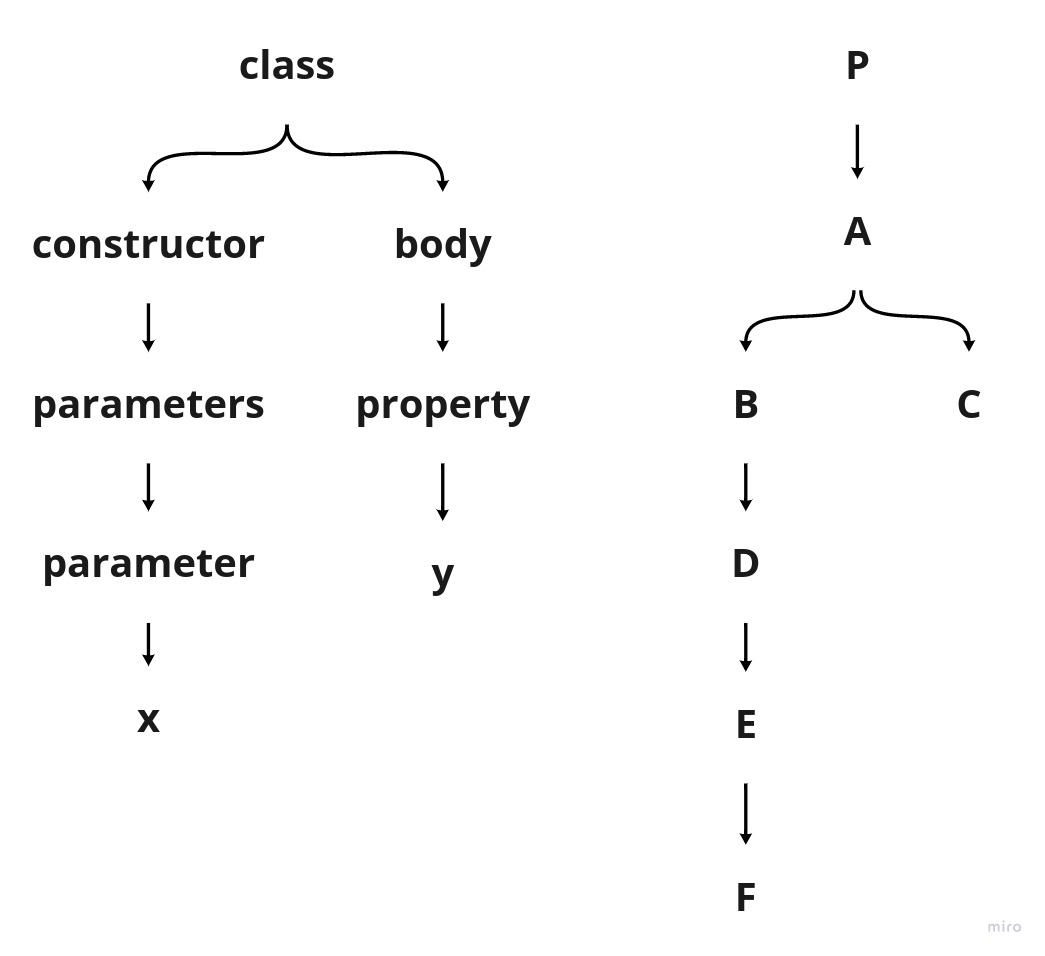
\includegraphics[width=0.6\textwidth]{deep.jpg}
\end{figure}

\subsection{Графовые нейронные сети}\label{sec:gnn}
Значительно более мощным является подход с использованием графовых нейронных сетей (Graph Neural Network - GNN). Каждой вершине сопостовляется вектор состояния, после чего происходит несколько этапов обмена информации между вершинами. Этап состоит из двух фаз: отправка сообщений и получение сообщений. Во время первой фазы для каждой вершины вычисляется сообщение для отправки. В качестве сообщения используется вектор состояния, преобразованный каким-либо образом. После того как все сообщения вычислины, вершины передают сообщения своим соседям, начинается вторая фаза. Во время фазы получения сообщений каждая вершина агрегирует получаемые от других вершин сообщения, например, в работе~\cite{graph-attention-networks} сообщения взвешенно усреднются с использованием механизма внимания. Состояние вершины обновлятеся с помощью полученного только что агрегированного сообщения. Это можно сделать, например, с помощью конкетенации этих векторов и линейного предобразования для уменьшения размерности конкатенированного вектора до исходной размерности состояния вершины.

Простой вариант - использовать AST в качестве графа. Однако в статье~\cite{gated-graphs-nn} предлагается дополнить этот граф ребрами data-flow графа. Например, можно соеденить вызов функции и возвращаемое значение из опредленение функции или аргументы вызова с параметрами функции. В таком случае информация по графовой нейронной сети в некоторых случаях будет передаваться также как и в исходном коде.

\subsection{Дерево разбора как список правил}\label{sec:treegen}
Дерево разбора можно представить в виде последовательности, но значительно хитрее, чем в описанном ранее случае, где дерево заменялось на список вершин в порядке обхода в глубину. Подход, используемый в статье~\cite{tree-gen} рассматривает синтаксическое дерево как последовательность приминения правил грамматики.

\begin{figure}[!h]
    \caption{Слева некоторые правила грамматики, справа - дерево, получающееся при последовательном применении правил 1, 7, 12, 20}\label{treegen}
    \centering
    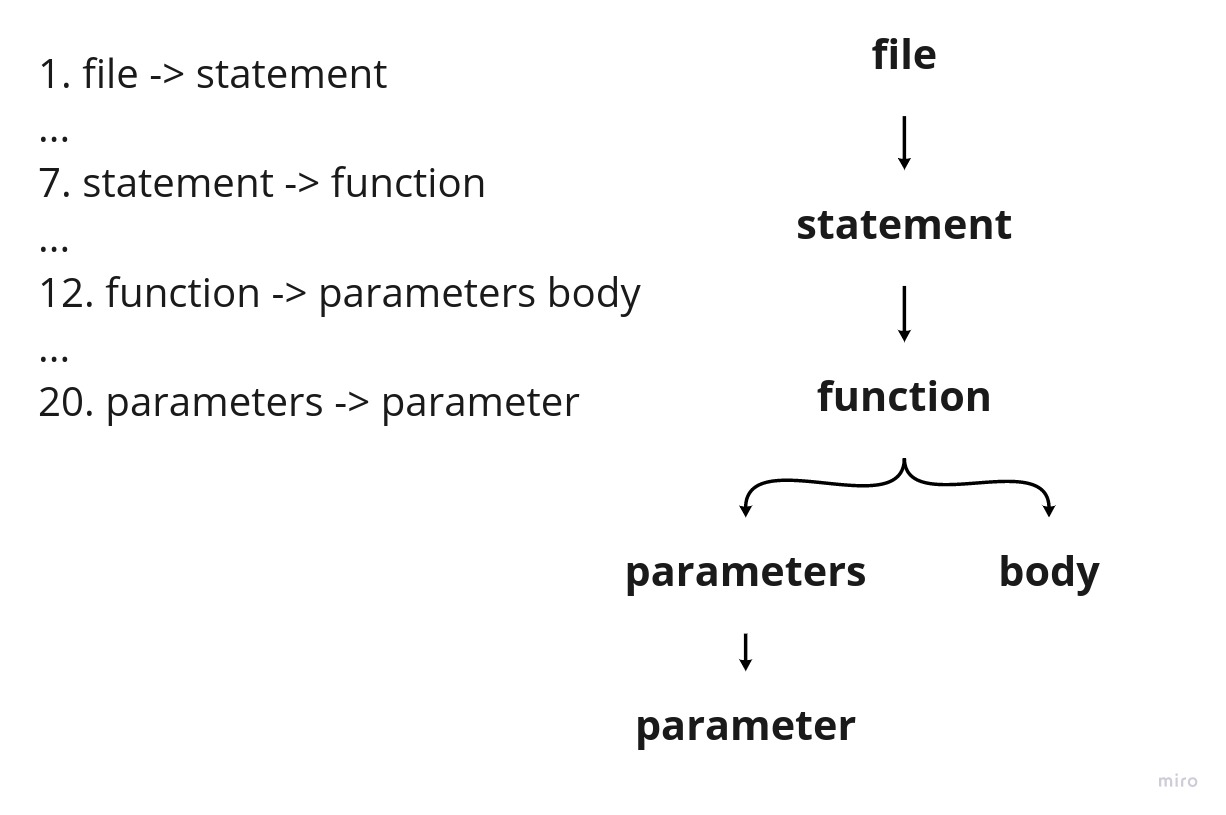
\includegraphics[width=0.7\textwidth]{treegen.jpg}
\end{figure}

Рассмотрим пример. Слева на рисунке~\ref{treegen} указаны некоторые правила грамматики. Будем считать, что \texttt{file} - это стартовый нетерминал, тогда после использования правил 1, 7, 12, 20 дерево примет вид изображенный справа на том же рисунке. В качестве текущего нетерминала для раскрытия выбирается первый в порядке обхода в глубину. То есть следующее правило будет раскрывать нетерминал \texttt{parameter}. Такое решение описывает исходный код очень близко к грамматике.

\subsection{Дерево разбора как набор путей}\label{sec:slm}
Еще один подход для представления дерева разбора кода рассмотрен в статье~\cite{code2vec}. При таком способе AST представляется в виде набора путей между всеми парами вершин в дереве. Далее эбмединги путей проходят через блок трансформера, механизм внимания позволяет выделить наиболее важные пути, после чего они взвешенно суммируются. Таким образом вычислятеся векторное представление примера кода.

Логику этого подхода продолжает статья~\cite{slm}. Там ставится задача дополнения кода (code completion), то есть предсказания вершины по контексту. В качестве входных данных на очередном шаге используются пути от всех листьев до родителя предсказываемой вершины, а также путь от корня дерева.

\begin{figure}[!h]
    \caption{Несколько шагов работы модели по дополнению кода}\label{slm}
    \centering
    \includegraphics[width=1\textwidth]{slm.jpg}
\end{figure}

На рисунке~\ref{slm} демострируется несколько шагов такого подхода. За \texttt{???} обозначается вершина, которую необходимо предсказать, к ее родителю идут зеленые стрелки, показывающие пути от листьев. Интересно отметить переход от второй картинки к третьей. На втором шаге было предсказан \texttt{x} - ребенок вершины \texttt{reference}. Так как \texttt{x} является листом, то модель прекращет генерацию в этом поддереве и начитает собирать пути ко второму ребенку \texttt{binary expr}. Важным моментом является то, что также учитывается путь от только что сгенерированного поддерева с \texttt{reference} и \texttt{x}.

\colorbox{orange}{нужно рассказать что-то про трансформеры}

\section{Подходы к извлечению семантической информации}\label{sec:semantic}
Ранее описанные механизмы делают больший акценкт на синтаксис языка, за исключением некоторых деталей. Как уже было сказано, ислючить семантику совсем нельзя, а значит данные модели самостоятельно обучаются семантике. Рассмотрим некоторые способы непосредственной передачи семантической информации модели.

\subsection{Семантические ребра}\label{sec:semanticEdges}
В обзоре подхода из статьи~\cite{gated-graphs-nn} уже было сказано о том, что графовая нейронная сеть обучается не просто на дереве разбора кода, а на его расшрении за счет ребер из data-flow графа. По идее такой способ представления кода должен способствовать усвоению не только синтаксической информации (за счет использования AST), но и семантической (за счет ребер data-flow графа).

Также в данной статье присутствует способ работы с типами для случая статически типизируемых языков, когда типы выражений известны на этапе компиляции. Для каждого типа предлагается использовать обучаемое векторное представление. Эмбедингом типа считается максимальное значение среди таких представлений для самого типа и его родительских типов. Использование операции максимум по сути позволяет обучить решетку на типах, то есть упорядочить их в иерархию.

\subsection{Предсказание типов}\label{sec:lambdanet}
Использование в~\cite{gated-graphs-nn} информации о типах наталкивает на мысль о важности этих данных. Действительно, знание типов в процессе разработки значительно помогает программисту - так разработчик понимает устройство сущности с которой он работает не только из ее названия, но и из структурного описания. 

\colorbox{orange}{рассказ о LambdaNet}


\section{Улучшение модели}\label{sec:improve}
Практически во всех указанных работах модели не используют напрямую семантическую информацию. Исключением является статья~\cite{gated-graphs-nn} о применении графовых нейронных сетей для представления исходного кода, где внедряют информацию о типах объектов, обучая решетку на типах. Такой подход позволяет частично сохранить иерархию типов, даже для новых типов, не видимых на этапе обучения. Однако типы определяются не только иерархией. Кроме нее, есть как минимум поля и методы, которые можно вызвать на экземпляре класса.

Важно отметить, что информация о типе не является чем-то недоступным, ее можно получить на этапе компиляции. Поэтому лучше попытаться использовать имеющуюся информацию, чем надеятся, что модель самостоятельно ее распознает и выучит.

Таки образом ставится задача разработать и внедрить механизмы работы с семантикой в модель, в частности для передачи более сложной информации о типах выражений.

\chapterconclusion
В данной главе рассматриваются некоторые спосбы представления исходного кода программы для работы с моделями машинного обучения, а также подходы к извлечению семантической инфорации из кода.


\chapter{Обработка семантики}

В данной главе будет выбрана базовая модель для последющего улучшения. Также будут предложены подходы для ее расширения с целью использования семантичекой информации.

\section{Выбор модели}\label{sec:chooseModel}
Для задачи генерации кода графовые нейронные сети не самый лучший вариант. Во-первых, не приминялись \colorbox{orange}{??}. Во-вторых, они тяжело учатся \colorbox{orange}{??}.

Подход со списком правил выглядит неплохим вариантом, но \colorbox{orange}{что?} можно сказать что он постарее, чем SLM и нигде(?) больше не применялся. Тем не менее его можно рассмотреть в дальнейших исследованиях.

В данной работе в качестве основы выбран подход из статьи \colorbox{orange}{Structural} language models of code. В целом подход себя зарекомендовал для решения таких задач как предсказание имени метода и генерация описания кода на естественном языке. Более того, конкретно в этой статье подход используется для генерации (пусть и небольших фрагментов) кода.

\colorbox{orange}{Генерация среднего кода. Почему это не плохо} - статья Даниила

\section{Интерграция типов}\label{typeIntro}
Типы в языках программирования устроены как правило достаточно сложным образом. Поэтому необходимо выбрать некоторое упрощенное описание типов и на его основе разработать и обучить модель. Каким же образом можно описать типы? В первом приближении тип описывается набором супертипов, а также его членами - методами и полями. Однако, есть и более сложные моменты - inner классы, вложенные классы, типовые параметры и многое другое, но в данной работе они не рассматриваются.

\subsection{Особенности описания типов}\label{typeDescr}
Даже с таким описанием класса встречаются интересные ситуации. Например, наличие возможности переопределения полей и методов в классах-наследниках. В таком случае информация об этих сущностях будет содержаться и в родительском классе и в наследнике. Для избежания дублирования информации есть следующее предложение: давайте будем игнорировать все переопределения. Инфомация о наличии метода с определенной сигнатурой или поля определенного типа в любом случае есть в описании родительского класса.

Другой интересный вопрос - это имена классов. Есть ли разница между классами \texttt{A} и \texttt{B} в листинге~\ref{lst2}? С одной стороны они абслютно идентичны в структурном плане и нет необходимости различать их как два различных типа - с экземпляром каждого из них можно делать один и тот же набор действий. С другой стороны такой подход имеет слабое место, например, экземляр \texttt{d} класса \texttt{D} можно привести к супертипу \texttt{A}, который, как сказано ранее эквивалентен классу \texttt{B}, а значит в таком подходе валидно приведение типа \texttt{d as E}, хотя в иерархии классов \texttt{D} и \texttt{E} расположены в разных местах. Тем не менее это не должно приводить к некомпилируемым результатам, поэтому мы пренебрежем данной особенностью.

\begin{lstlisting}[float=!h,caption={Пример исходного кода на Kotlin},label={lst2}]
class A(val x: Int)
class B(val y: Int)
class C(val x, Int, val y: Int)
class D(val y: Int) : A(100)
class E(val z: Double) : B(100)
\end{lstlisting}

Отметим, что классы \texttt{C} и \texttt{D} будут считаться различным, не смотря на то, что оба содержат два поля типа \texttt{Int} (\texttt{C} напрямую, \texttt{D} - один напрямую, а второй через наследоавние от \texttt{А}).

Выходит, что формулируемый подход описывает класс с точки зрения того, что можно делать с его экземпляром - какие методы вызывать и к полям какого типа обращаться. Однако, наличие у класса членов с модификаторами \texttt{private} и \texttt{protected} совсем не сочитаются с данным подходом из-за того, что доступа к ним из вне класса нет. Заметим, что наличие для приватного поля публичных методов для его модификации наполнит описание класса информацией ровно об этих методах, но не о соответсвующем поле. Вопрос что конкретно делают эти методы, действительно ли что-то модифицируют не имеет смысла в рамках поставленной задачи. Понимая, что \texttt{private} и \texttt{protected} члены класса не играют важной роли, а возможно даже вредят, мы исключим информарцию о них из описания класса.

\subsection{Определение порядка построения эмбедингов типов}\label{order}
Вновь обращаясь к листингу~\ref{lst2} заметим, что нет особого смысла создавать эмбединг сначала для класса \texttt{D}, а только потом для класса \texttt{A}, ведь \texttt{D} должен содержить информацию о классе \texttt{A}. Сразу на ум приходит разумная идея - давайте посторим граф зависимостей типов, проведем на вершинах топологическую сортировку и построим эмбединги типов в порядке обратном данной сортировке.

Однако такой граф будет содержать циклы, что делает построение сортировки невозможным. Примеры "плохого" кода представлены в листинге~\ref{lst3}. В первом случае \texttt{Tree} - обычный рекурсивный тип, порождающий петлю в графе зависимостей. Во втором случае ни \texttt{A}, ни \texttt{B} не являются рекурсивными сами по себе, но образуют циклическую зависимость, ссылаясь друг на друга. В последнем примере класс \texttt{D} не имеет ни одного поля непостредственно, но становится рекурсивным из-за наследования от класса \texttt{C}, содержащего поля типа \texttt{D}.

\begin{lstlisting}[float=!h,caption={Типы с циклическими зависимостями},label={lst3}]
class Tree(var t: Tree?)

class A(var b: B?)
class B(var a: A?)

class C(var d: D?)
class D : C
\end{lstlisting}

\colorbox{orange}{Нужна оценка на долю рекурсивных классов}
Так как доля таких ситуаций крайне мала, предлагается просто исключить все рекурсивные зависимости, а именно удалять одно из ребер, в каждом цикле. Важно понимать, что после того как класс лишается зависимости на какой-либо тип, он больше не может содержать поля такого типа, а его функции-члены не могут иметь этот типа в качестве параметра или возвращаемого значения. Такие члены класса придется удалить. После указанного преобразования представления классов будут менее точными, но все еще насыщенными большим объемом информации.

При внимательном рассмотрении структуры типа \texttt{Any}, а также примитивных типов становится ясно, что все они содержат рекурсивные зависимости. Например, \texttt{Any} содержит метод \texttt{equals: (Any?)  $\rightarrow$ Boolean}, что создает один цикл с самим собой и еще один цикл с классом \texttt{Boolean}. А любой числовой тип содержит в частности методы \texttt{compareTo(X)}, где в качестве \texttt{X} может быть любой из числовых типов \texttt{Byte, Short, Int, Long, Float, Double}. 

Лишаться информации об этих методах совсем не хочется, поэтому предгалается следующее решение. Определим набор базовых типов, которые будут своего рода кирпичиками при построении более сложных типов. В этот набор войдут числовые типы - \texttt{Byte, Short, Int, Long, Float, Double}, типы, связанные со строками - \texttt{Char, CharSequence}, логический тип \texttt{Boolean} и типы общего вида \texttt{Any, Unit}. Так как для базовых типов постороение эмбедингов исходя из структуры этих классов невозможно по причине рекурсивных зивисимостей, эмбеденги будут предложены напрямую. При этом информация о их методах будет использована в процессе обучения для корректировки их векторных представлений.

Типы из выбранного базового набора можно запросто увидеть в любой программе, более того этот набор ограничен, а значит не должно возникнуть проблемы с обучением эмбедингов для этих типов. Важно, что такой подход никак не поможет для других типов с циклическими зависимостями - их пространство слишком велико, и мы не можем выдать всем им эмбединги напрямую.

\subsection{Алгоритм построения эмбедингов типов}\label{typeEmbAlgo}
Для конструирования модели для эмбедингов типов небходимо ответить на следующие вопросы в общем случае: ``сколько параметров в функции?'', ``сколько членов в классе?'', ``сколько супертипов имеет класс?''. Ответ оказывается достаточно простым - сколько угодно. В виду отсутствия каких-либо ограничений предлагается использовать реккурентные нейронные сети для сбора информации о параметрах, членах класса и супертипах. Так как в каждом таком случае информация может иметь разные свойства, будем использовать три различных нейронных сети с разными весами.

Опишем алгоритм более строго:
\begin{enumerate}
    \item Для базовых типов выберем случайные обучаемые векторные предствления
    \item Для каждого класса построим его эмбединг, если это не сделано ранее:
    \begin{enumerate}
        \item Рекурсивно получим эмбединги для всех классов, от которых зависит текущий
        \item Построим эмбденги для всех функций членов текущего класса:
        \begin{enumerate}
            \item Пропустим через рекуррентную нейронную сеть все параметры, получая векторное представление списка параметров
            \item С помощью линейного преобразования объеденим вектороное предстваления списка параметров и возвращаемого типа
        \end{enumerate}
        \item Пропустим через вторую рекуррентную нейронную сеть эмбединги всех функций членов и эмбединги типов всех полей, получая вектороное предствление класса вне иерархии типов
        \item Пропустим через третью рекуррентную нейронную сеть эмбединги всех супертипов, а также эмбединг с предыдущего шага
    \end{enumerate}
\end{enumerate}

Стоит отметить, что не все классы содержат члены, и не все функции имеют хотя бы один параметр. Поэтому для корректной работы необходимы обучаемые вектора, означающие пустой список параметров и пустой список членов класса.

После выполнения алгоритма у нас имеются векторные представления для всех классов и функций в экземпляре исходного кода. Однако совершенно недостаточно получить случайные векторные представления, необходимо получить именно такие, которые сохраняют полезную информацию о типе. Проверка этой информации и будет основой при обучении. 

Мы обладаем некоторыми знаниями о всех типах, например, что тип \texttt{A} является подтипом \texttt{B} или что функция \texttt{F} возвращает значение типа \texttt{C}. Поэтому оценивать качество получившихся векторных предствалений типов можно на основе соответствующих вопросов - ``\texttt{A} подтип \texttt{B}?'', ``\texttt{F} возвращает \texttt{C}?'', решая задачу бинарной классификации.

При интеграции типов в основную модель нужно помнить о двух вещах. Во-первых, так как мы обладаем информацией о типах некоторых вершин в AST, например, тип вершины, отвечающей за вызов функции может соответсвтовать типу возвращаемого значения этой функции, хочется передавать эту информацию модели. Во-вторых, нужно каким-то образом получать результы на основе типов, например, для новых переменных можно предсказывать конкретный тип, чтобы указывать его при генерации подставлять его при генерации.

Исходя из этого предлагается для описания вершины в AST использовать конкатенацию векторного представления вида вершины (например, \texttt{RETURN} или \texttt{FUN}) и векторного представления типа, если он есть. Аналогичные изменения должны быть с выходом модели, то есть полученный вектор можно разбить на два - отвечающий за вид вершины и отвечающий за тип.

\section{Механизм обучения}\label{fit}
В оригинальной модели в качестве ожидаемого результата при обучении используется тот вид вершины, который был в изначальном примере. Такой подход не соответствует цели, поставленной в данной работе, поэтому необходимо изменить механизм обучения.

\subsection{Обучение синтаксису}\label{fit:syntax}
Первое, с чем приходится сталкиваться, это синтаксическая корректность - мы хотим, чтобы код был правильным с точки зрения грамматики. Поэтому будем штрафовать модель за предсказание заведомо не подходящих видов вершин. Соответсвенно, предсказаниямя с наибольшей вероятностью будут подходящими с точки зрения синтаксиса. 

Существуют такие случаи, когда добавление вершины в AST делает его синтаксически некорректным, однако при продолжении наращивания дерева ошибки пропадают. Примерами могу послужить операции доступа через точку \texttt{$\star$.$\star$} или бинарная операция \texttt{$\star$ + $\star$}. В обоих случаях за $\star$ обозначаются отсутствующие дети, необходимые для компилируемости кода.

Из-за того, что в ходе работы не обнаружено простого способа понять является ли добавление очередной вершины в дерево синтаксинтаксически некорректным в принципе, при любых дальнейших действиях, или только по причине необходимости наличия детей у нее самой, был реализован простой механизм такой проверки. Основываясь на датасете, определим следующее отношение: \{(A, B) | сущетсвует такое AST, в котором вершина вида A содержит как ребенка вершину вида B\}. Использовать его как критерий синтаксической корректности не очень надежно, например, оно не мешает иметь вершине вида \texttt{IF} сразу двух детей вида \texttt{CONDITION}.

Первое, что мы сделаем для усложения этого отношения будет использование информации о видах детей слева от предсказываемой вершины: \{(A, B, LB) | сущетсвует такое AST, в котором вершина вида A содержит как детей вершины видов LB, а затем вершину вида B\}. Такой подход позволит избавиться от ошибки, указанной выше, однако порождает новую: число различных комбинаций детей, например, у \texttt{FILE} крайне велико (в отличие от \texttt{IF}, который имеет только $[\varnothing]$, \texttt{[CONDITION]}, \texttt{[CONDITION, THEN]} и \texttt{[CONDITION, THEN, ELSE]}), а значит мы очень сильно ограничиваемся разнообразием датасета. Поэтому вторая модификация залючается в том, что для подобного рода вершин мы не будем требовать порядка на детях. Помимо \texttt{FILE} это коснется блоков кода, выражений \texttt{when}, строк (из-за интерполяции), списков параметров и аргументов значений и типов.

\subsection{Обучение семантике}\label{fit:syntax}
На самом деле проблема из предыдущего раздела про некомпилируемость кода из-за недостроенности дерева разброра не ограничивается синтаксисом. Рассмотрим пример из листинга~\ref{lst4}. Пусть решено инициализировать переменную с помощью условоного оператора, однако конструкция (2) не валидна даже с точки зрения синтаксиса, так как отсутвует условие. Но добавления условия тоже недостаточно, ведь \texttt{if} используется для инициализации и типы блоков \texttt{THEN} и \texttt{ELSE} должны соответствовать типу пемеменной \texttt{x}. Поможет только генерация всего поддерава вершины вида \texttt{IF}.

\begin{lstlisting}[float=!h,caption={Возможная последовательная генерация},label={lst4}]
(1) val x: Int = ???                             //не компилируется
(2) val x: Int = if (???) { ??? } else { ??? }   //не компилируется
(3) val x: Int = if (true) { ??? } else { ??? }  //не компилируется
(4) val x: Int = if (true) { 4 } else { ??? }    //не компилируется
(5) val x: Int = if (true) { 4 } else { 5 }      //компилируется
\end{lstlisting}

Исходя из этого примера, стратегия обучения должна давать возможность модели предсказать поддерево целиком. Если получен компилируемый результат, модель должна быть поощрена за свой выбор. Если результат не коспилируется, это может означать либо что полученный код не приводим к компилируемому ни при каких условиях, либо он пока еще не приведен, как в пунктах 2-4 в листинге~\ref{lst4}. Чтобы понять с чем мы столкнулись, дадим модели завершить несколько поддеревьев. Если даже после завершения нескольких поддеревьев код не стал компилируемым, значит высока вероятность, что он таким и не станет, и модель должна быть оштрафована за принятие своих решенией.

\section{Подход к оцениваю}\label{rate}
\colorbox{orange}{1. Метрики для генерации}

предсказываемая вершина vs оригинальная

обучить без семантики????

доля семантически-верного кода

\colorbox{orange}{2. Метрики для фаззинга}

запуск компилятора на сгенерированном (в т.ч. с разными параметрами)

время работы / число вершин

запуск под разными платформами

\chapterconclusion

В данной главе приянто и обосновано решение об использовании преставления исходоного кода на основе путей в дереве разбора, предложен механизм построения векторных представлений для типов и способ внедрения информации о типах в основную модель, описан способ обучения основной модели.


\chapter{Реализация и результаты}

\section{Реализация на стороне Kotlin'а}
\colorbox{orange}{кэширование деревьев, ALTree и извлечение путей}

\colorbox{orange}{Архитектура генератора}

\section{Особенности реализации модели для типов и результаты обучения}
Для формулирования задач бинарной классификации был выбран ряд логичных с точки зрения программирования вопросов, ответ на которые должен содержаться в эмбедингах типов. Для обучения было предложено несколько групп вопросов: наличие отношения наследования между типами, наличие определненных членов в классе, информация о возвращаемом значении функции. Для каждой группы создавалась для получения ответа на вопрос нейронная сеть, решаюшая задачу бинарной классификации. Для каждой группы формулировались вопросы, в том числе отличающиеся по виду аргументов. Для примера рассмотрим вопросы из последней группы:
\begin{enumerate}
    \item
        \begin{itemize}
            \item Ситуация: A возращает значение именно типа B
            \item Вопрос: ``А возвращает B''
            \item Ответ: ``да''
        \end{itemize}
    \item 
        \begin{itemize}
            \item Ситуация: A возращает значение типа C, C - подтип B, значит можно сказать, что A возращает значение типа B
            \item Вопрос: ``А возвращает B''
            \item Ответ: ``да''
        \end{itemize}
    \item 
        \begin{itemize}
            \item Ситуация: A возращает значение не типа B и не его подтипов
            \item Вопрос: ``А возвращает B''
            \item Ответ: ``нет''
        \end{itemize}
\end{enumerate}

Для того, чтобы не возникло переобучения модели на конкретный ответ, доля вопросов с ответами ``да'' и ``нет'' балансируется. Результаты оценки точности предсказания представлены в таблице~\ref{tab1}

\begin{table}[!h]
\caption{\colorbox{orange}{Таблица умножения с помощью \texttt{tabularx} (фрагмент)}}\label{tab1}
\centering
\begin{tabularx}{\textwidth}{|*{18}{>{\centering\arraybackslash}X|}}\hline
Группа вопросов & Всего вопросов с ответом ``да'' & Всего вопросов с ответом ``нет'' & Средняя точность предсказаний для ответа ``да'' & Средняя точность предсказаний для ответа ``нет'' \\\hline
A - подтип B  & 2097 & 1847 & 0,943 & 0,918 \\\hline
A содержит B как член & 1458 & 1472 & 0,675 & 0,780 \\\hline
\colorbox{orange}{A - параметр B}  & 362 & 2133 & 0,567 & 0,955 \\\hline
A возвращает B & 2100 & 2164 & 0,858 & 0,845 \\\hline
\end{tabularx}
\end{table}

\section{Результат работы генератора}
\colorbox{orange}{Результат генерации кода}

\section{Возможные улучшения}
Для сохранения информации о типах выражений можно использовать более продвинутые подходы, например, на основе графовых нейронных сетей. Это позволит сохранять больше информации, в частности может позволить поддержать рекурсивные типы.

Также в ходе работы возникала, но не была реализована следующая идея. По аналогии с подходом из работы  \colorbox{orange}{ссылка}, где в дерево разбора добавлялись ребра, означающие семантические связи, хотелсь бы поддержать нечто подобное и в подходе на основе путей. Например, можно приминять к связанным вершинам некоторый оператор.

\begin{lstlisting}[float=!h,caption={Примеры семантических операторов},label={lst100}]
(1) typed_node = node_with_type(node, type)

(2) private_node = is_private_node(old_node)
(3) new_call, new_return = call_return(old_call, old_return)
(4) new_param, new_arg = param_arg(old_param, old_arg)
\end{lstlisting}

Обратимся к листингу~\ref{lst100}. В первой строке представлен оператор типизации вершины, по сути именно такой и используется в данной работе, однако три другие оператора - нет. Оператор (2) должен передать в вершину информацию о том, что она приватная. Для всех пар вызова и декларации соответсвующего метода можно приминить преобразование (3). То же касается и парных аргументов и параметров в случае оператора (4). Предполагается, что таким образом удастся внедрить дополнительную информацию в модель.

\chapterconclusion
фывфв


%% Макрос для заключения. Совместим со старым стилевиком.
\startconclusionpage

В данном разделе размещается заключение.

\printmainbibliography

\end{document}

